\documentclass[tikz,border=6pt]{standalone}
\usepackage{helvet}
\renewcommand{\familydefault}{\sfdefault}
\usetikzlibrary{decorations.pathmorphing}
\begin{document}
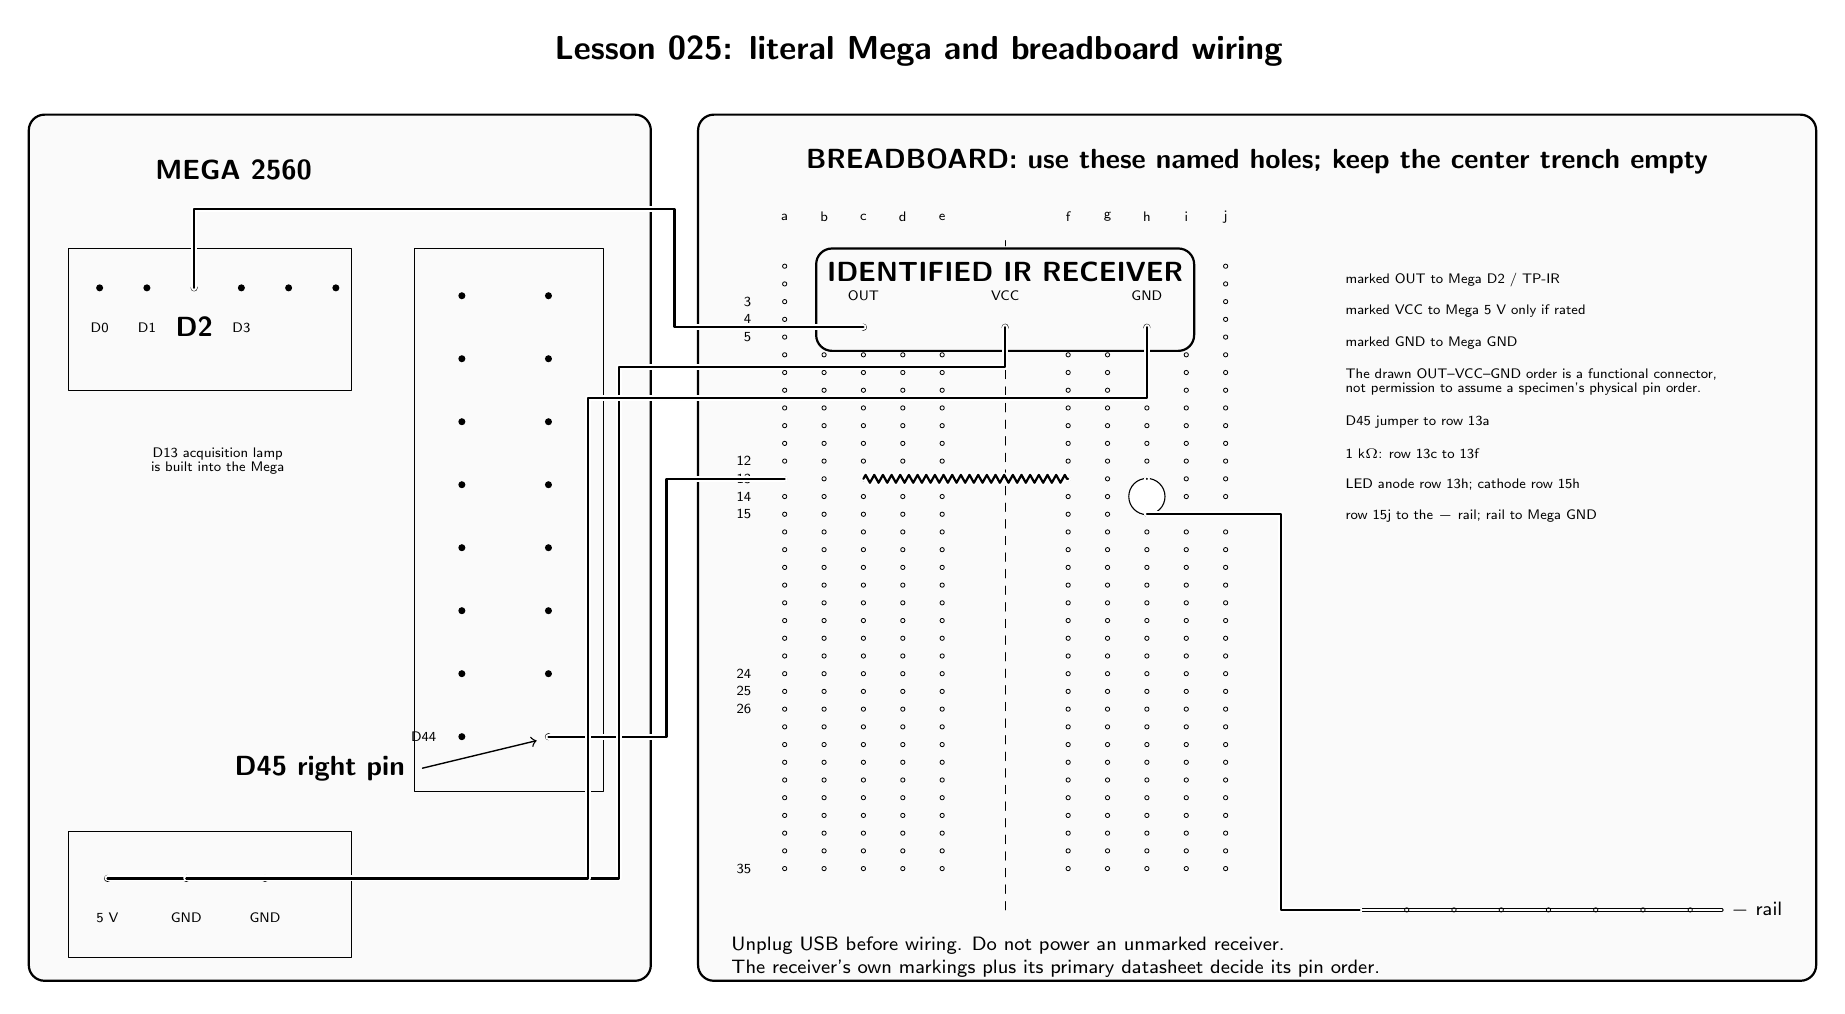
\begin{tikzpicture}[x=1mm,y=1mm,line cap=round,line join=round,
  board/.style={draw,line width=.8pt,rounded corners=2mm,fill=black!2},
  hole/.style={circle,draw,line width=.3pt,inner sep=.55pt},
  pin/.style={circle,fill=black,inner sep=.9pt},
  wire/.style={preaction={draw=white,line width=2.2pt},line width=.8pt},
  tiny/.style={font=\fontsize{4.7}{5.1}\selectfont},
  small/.style={font=\scriptsize}]

\node[font=\bfseries\large] at (116,126)
  {Lesson 025: literal Mega and breadboard wiring};

% Mega orientation and the occupied physical header positions.
\draw[board] (3,8) rectangle (82,118);
\node[font=\bfseries] at (29,111) {MEGA 2560};
\draw (52,32) rectangle (76,101);
\foreach \r in {0,...,7}
{
  \pgfmathsetmacro{\yy}{95-\r*8}
  \node[pin] at (58,\yy) {};
  \node[pin] at (69,\yy) {};
}
\node[tiny,anchor=east] at (56,39) {D44};
\node[tiny,font=\bfseries,anchor=east] at (52,35) {D45 right pin};
\draw[->,line width=.5pt] (53,35)--(67.5,38.5);
\draw (8,83) rectangle (44,101);
\foreach \x in {12,18,...,42}\node[pin] at (\x,96) {};
\node[tiny] at (12,91) {D0};
\node[tiny] at (18,91) {D1};
\node[tiny,font=\bfseries] at (24,91) {D2};
\node[tiny] at (30,91) {D3};
\node[tiny,align=center] at (27,74) {D13 acquisition lamp\\is built into the Mega};
\draw (8,11) rectangle (44,27);
\node[pin] at (13,21) {};\node[pin] at (23,21) {};\node[pin] at (33,21) {};
\node[tiny] at (13,16) {5 V};\node[tiny] at (23,16) {GND};\node[tiny] at (33,16) {GND};

% Literal breadboard, center trench, numbered rows, and power rail.
\draw[board] (88,8) rectangle (230,118);
\node[small,font=\bfseries] at (159,112)
  {BREADBOARD: use these named holes; keep the center trench empty};
\foreach \c/\x in {a/99,b/104,c/109,d/114,e/119,f/135,g/140,h/145,i/150,j/155}
  \node[tiny] at (\x,105) {\c};
\draw[dashed] (127,17)--(127,102);
\foreach \r in {1,...,35}
{
  \pgfmathsetmacro{\yy}{101-\r*2.25}
  \foreach \x in {99,104,109,114,119,135,140,145,150,155}
    \node[hole] at (\x,\yy) {};
}
\foreach \r in {3,4,5,12,13,14,15,24,25,26,35}
{
  \pgfmathsetmacro{\yy}{101-\r*2.25}
  \node[tiny,anchor=east] at (96,\yy) {\r};
}
\draw[double] (169,17)--(218,17);
\node[small,anchor=west] at (218,17) {$-$ rail};
\foreach \x in {172,178,...,214}\node[hole] at (\x,17) {};

% Evidence LED path: D45 -> resistor -> anode, cathode -> ground.
\draw[wire] (69,39)--(84,39)--(84,71.75)--(99,71.75);
\draw[wire,decorate,decoration={zigzag,segment length=1.1mm,amplitude=.5mm}]
  (109,71.75)--(135,71.75);
\draw[fill=white] (145,69.5) circle (2.3);
\draw[wire] (145,71.75)--(145,71.75);
\draw[wire] (145,67.25)--(162,67.25)--(162,17)--(172,17);
\node[tiny,anchor=west] at (169,79)
  {D45 jumper to row 13a};
\node[tiny,anchor=west] at (169,75)
  {1 k$\Omega$: row 13c to 13f};
\node[tiny,anchor=west] at (169,71)
  {LED anode row 13h; cathode row 15h};
\node[tiny,anchor=west] at (169,67)
  {row 15j to the $-$ rail; rail to Mega GND};

% Identified receiver: each functional pin gets a distinct row.
\draw[board] (103,88) rectangle (151,101);
\node[tiny,font=\bfseries] at (127,98) {IDENTIFIED IR RECEIVER};
\node[pin] at (109,91) {};\node[pin] at (127,91) {};\node[pin] at (145,91) {};
\node[tiny] at (109,95) {OUT};
\node[tiny] at (127,95) {VCC};
\node[tiny] at (145,95) {GND};
\draw[wire] (24,96)--(24,106)--(85,106)--(85,91)--(109,91);
\draw[wire] (13,21)--(78,21)--(78,86)--(127,86)--(127,91);
\draw[wire] (23,21)--(74,21)--(74,82)--(145,82)--(145,91);
\node[tiny,anchor=west] at (169,97) {marked OUT to Mega D2 / TP-IR};
\node[tiny,anchor=west] at (169,93) {marked VCC to Mega 5 V only if rated};
\node[tiny,anchor=west] at (169,89) {marked GND to Mega GND};
\node[tiny,anchor=west,align=left] at (169,84)
  {The drawn OUT--VCC--GND order is a functional connector,\\
   not permission to assume a specimen's physical pin order.};

\node[small,align=left,anchor=west] at (91,11)
  {Unplug USB before wiring. Do not power an unmarked receiver.\\
   The receiver's own markings plus its primary datasheet decide its pin order.};
\end{tikzpicture}
\end{document}
